\documentclass[12pt, a4paper,  BCOR=8.25mm, DIV=15]{scrartcl}\usepackage[]{graphicx}\usepackage[]{color}
%% maxwidth is the original width if it is less than linewidth
%% otherwise use linewidth (to make sure the graphics do not exceed the margin)
\makeatletter
\def\maxwidth{ %
  \ifdim\Gin@nat@width>\linewidth
    \linewidth
  \else
    \Gin@nat@width
  \fi
}
\makeatother

\definecolor{fgcolor}{rgb}{0.345, 0.345, 0.345}
\newcommand{\hlnum}[1]{\textcolor[rgb]{0.686,0.059,0.569}{#1}}%
\newcommand{\hlstr}[1]{\textcolor[rgb]{0.192,0.494,0.8}{#1}}%
\newcommand{\hlcom}[1]{\textcolor[rgb]{0.678,0.584,0.686}{\textit{#1}}}%
\newcommand{\hlopt}[1]{\textcolor[rgb]{0,0,0}{#1}}%
\newcommand{\hlstd}[1]{\textcolor[rgb]{0.345,0.345,0.345}{#1}}%
\newcommand{\hlkwa}[1]{\textcolor[rgb]{0.161,0.373,0.58}{\textbf{#1}}}%
\newcommand{\hlkwb}[1]{\textcolor[rgb]{0.69,0.353,0.396}{#1}}%
\newcommand{\hlkwc}[1]{\textcolor[rgb]{0.333,0.667,0.333}{#1}}%
\newcommand{\hlkwd}[1]{\textcolor[rgb]{0.737,0.353,0.396}{\textbf{#1}}}%

\usepackage{framed}
\makeatletter
\newenvironment{kframe}{%
 \def\at@end@of@kframe{}%
 \ifinner\ifhmode%
  \def\at@end@of@kframe{\end{minipage}}%
  \begin{minipage}{\columnwidth}%
 \fi\fi%
 \def\FrameCommand##1{\hskip\@totalleftmargin \hskip-\fboxsep
 \colorbox{shadecolor}{##1}\hskip-\fboxsep
     % There is no \\@totalrightmargin, so:
     \hskip-\linewidth \hskip-\@totalleftmargin \hskip\columnwidth}%
 \MakeFramed {\advance\hsize-\width
   \@totalleftmargin\z@ \linewidth\hsize
   \@setminipage}}%
 {\par\unskip\endMakeFramed%
 \at@end@of@kframe}
\makeatother

\definecolor{shadecolor}{rgb}{.97, .97, .97}
\definecolor{messagecolor}{rgb}{0, 0, 0}
\definecolor{warningcolor}{rgb}{1, 0, 1}
\definecolor{errorcolor}{rgb}{1, 0, 0}
\newenvironment{knitrout}{}{} % an empty environment to be redefined in TeX

\usepackage{alltt}
\usepackage[utf8]{inputenc}
\usepackage{newfloat}
\DeclareFloatingEnvironment[name={Supplementary Figure}]{suppfigure}

\newenvironment{itemizz}%
  {\begin{itemize}%
    \setlength{\itemsep}{2pt}%
    \setlength{\parskip}{2pt}}%
  {\end{itemize}}

\newcommand{\txtt}[1]{{\texttt{#1}}}
\IfFileExists{upquote.sty}{\usepackage{upquote}}{}
\begin{document}
%\VignetteEngine{knitr::knitr}
%\VignetteIndexEntry{Brief Notes on Text Mining (Set 14)}



\title{14: Brief Notes on Text Mining}
\author{John H Maindonald}
\maketitle
\vspace*{-0.5cm}

\begin{knitrout}
\definecolor{shadecolor}{rgb}{0.969, 0.969, 0.969}\color{fgcolor}\begin{kframe}
\begin{alltt}
\hlstd{doFigs} \hlkwb{<-} \hlnum{TRUE}
\end{alltt}
\end{kframe}
\end{knitrout}
\vspace*{-0.5cm}

Load the {\em DAAGviz} package:
\begin{knitrout}
\definecolor{shadecolor}{rgb}{0.969, 0.969, 0.969}\color{fgcolor}\begin{kframe}
\begin{alltt}
\hlkwd{library}\hlstd{(DAAGviz,} \hlkwc{quietly}\hlstd{=}\hlnum{TRUE}\hlstd{)}
\end{alltt}
\end{kframe}
\end{knitrout}

Set up a path to the directory where texts (.pdf and .txt)
are stored:
\begin{knitrout}
\definecolor{shadecolor}{rgb}{0.969, 0.969, 0.969}\color{fgcolor}\begin{kframe}
\begin{alltt}
\hlcom{## Create paths to the files}
\hlstd{txdir} \hlkwb{<-} \hlkwd{system.file}\hlstd{(}\hlkwc{package}\hlstd{=}\hlstr{'DAAGviz'}\hlstd{,} \hlstr{"texts"}\hlstd{)}
\hlkwd{print}\hlstd{(}\hlkwd{dir}\hlstd{(txdir,} \hlkwc{pattern}\hlstd{=}\hlstr{".txt$"}\hlstd{))}
\end{alltt}
\begin{verbatim}
[1] "data6-7.txt"     "graphics8-9.txt"
[3] "prelims1-5.txt" 
\end{verbatim}
\begin{alltt}
\hlstd{txfiles} \hlkwb{<-} \hlkwd{dir}\hlstd{(txdir,} \hlkwc{pattern}\hlstd{=}\hlstr{".txt$"}\hlstd{,} \hlkwc{full.names}\hlstd{=}\hlnum{TRUE}\hlstd{)}
\end{alltt}
\end{kframe}
\end{knitrout}

Choose a color palette:

\begin{knitrout}
\definecolor{shadecolor}{rgb}{0.969, 0.969, 0.969}\color{fgcolor}\begin{kframe}
\begin{alltt}
\hlstd{pal} \hlkwb{<-} \hlstd{RColorBrewer}\hlopt{::}\hlkwd{brewer.pal}\hlstd{(}\hlnum{6}\hlstd{,} \hlstr{"Dark2"}\hlstd{)}
\end{alltt}
\end{kframe}
\end{knitrout}

\begin{knitrout}
\definecolor{shadecolor}{rgb}{0.969, 0.969, 0.969}\color{fgcolor}\begin{kframe}
\begin{alltt}
\hlstd{dirSource} \hlkwb{<-} \hlstd{tm}\hlopt{::}\hlkwd{DirSource}\hlstd{(}\hlkwc{directory}\hlstd{=txdir,}
                       \hlkwc{pattern}\hlstd{=}\hlstr{".txt$"}\hlstd{)}
\end{alltt}
\end{kframe}
\end{knitrout}

\begin{knitrout}
\definecolor{shadecolor}{rgb}{0.969, 0.969, 0.969}\color{fgcolor}\begin{kframe}
\begin{alltt}
\hlstd{txcorp} \hlkwb{<-} \hlstd{tm}\hlopt{::}\hlkwd{Corpus}\hlstd{(dirSource)}
\hlstd{txcorp} \hlkwb{<-} \hlstd{tm}\hlopt{::}\hlkwd{tm_map}\hlstd{(txcorp,}
                 \hlstd{tm}\hlopt{::}\hlkwd{content_transformer}\hlstd{(}
                     \hlkwa{function}\hlstd{(}\hlkwc{x}\hlstd{)} \hlkwd{iconv}\hlstd{(x,} \hlkwc{to}\hlstd{=}\hlstr{"UTF-8"}\hlstd{,}
                                       \hlkwc{sub} \hlstd{=} \hlstr{"byte"}\hlstd{)),}
                 \hlkwc{mc.cores}\hlstd{=}\hlnum{1}\hlstd{)}
\end{alltt}
\end{kframe}
\end{knitrout}
\begin{knitrout}
\definecolor{shadecolor}{rgb}{0.969, 0.969, 0.969}\color{fgcolor}\begin{kframe}
\begin{alltt}
\hlstd{ctl} \hlkwb{<-} \hlkwd{list}\hlstd{(}\hlkwc{stopwords} \hlstd{=} \hlkwd{c}\hlstd{(tm}\hlopt{::}\hlkwd{stopwords}\hlstd{(),} \hlstr{"[1]"}\hlstd{),}
            \hlkwc{removePunctuation} \hlstd{=} \hlkwd{list}\hlstd{(}\hlkwc{preserve_intra_word_dashes} \hlstd{=} \hlnum{FALSE}\hlstd{),}
            \hlkwc{removeNumbers} \hlstd{=} \hlnum{TRUE}\hlstd{,} \hlkwc{stopwords}\hlstd{=}\hlkwd{c}\hlstd{(tm}\hlopt{::}\hlkwd{stopwords}\hlstd{(),} \hlstr{"[1]"}\hlstd{),}
            \hlkwc{minDocFreq} \hlstd{=} \hlnum{2}\hlstd{)}
\hlstd{tx.tdm} \hlkwb{<-} \hlstd{tm}\hlopt{::}\hlkwd{TermDocumentMatrix}\hlstd{(txcorp,} \hlkwc{control}\hlstd{=ctl)}
\end{alltt}
\end{kframe}
\end{knitrout}
\begin{knitrout}
\definecolor{shadecolor}{rgb}{0.969, 0.969, 0.969}\color{fgcolor}\begin{kframe}
\begin{alltt}
\hlstd{figset14} \hlkwb{<-} \hlkwa{function}\hlstd{()\{}
  \hlkwa{if}\hlstd{(}\hlopt{!}\hlkwd{requireNamespace}\hlstd{(}\hlstr{'tm'}\hlstd{,} \hlkwc{quietly} \hlstd{=} \hlnum{TRUE}\hlstd{))}\hlkwd{stop}\hlstd{(}\hlstr{'tm must be installed'}\hlstd{)}
  \hlkwa{if}\hlstd{(}\hlopt{!}\hlkwd{requireNamespace}\hlstd{(}\hlstr{'wordcloud'}\hlstd{,} \hlkwc{quietly}\hlstd{=}\hlnum{TRUE}\hlstd{))}\hlkwd{stop}\hlstd{(}\hlstr{'wordcloud must be installed'}\hlstd{)}
  \hlstd{\}}
\end{alltt}
\end{kframe}
\end{knitrout}

\begin{knitrout}
\definecolor{shadecolor}{rgb}{0.969, 0.969, 0.969}\color{fgcolor}\begin{kframe}
\begin{alltt}
\hlkwd{figset14}\hlstd{()}
\end{alltt}
\end{kframe}
\end{knitrout}


\begin{knitrout}
\definecolor{shadecolor}{rgb}{0.969, 0.969, 0.969}\color{fgcolor}\begin{kframe}
\begin{alltt}
\hlstd{doTDM} \hlkwb{<-} \hlkwa{if}\hlstd{(}\hlkwd{exists}\hlstd{(}\hlstr{"tx.tdm"}\hlstd{))} \hlnum{FALSE} \hlkwa{else} \hlnum{TRUE}
\hlstd{doCorp} \hlkwb{<-} \hlkwa{if}\hlstd{(doTDM} \hlopt{& !}\hlkwd{exists}\hlstd{(}\hlstr{"tx.corp"}\hlstd{))} \hlnum{TRUE} \hlkwa{else} \hlnum{FALSE}
\hlkwa{if}\hlstd{(doCorp)\{}
\hlstd{dirSource} \hlkwb{<-} \hlstd{tm}\hlopt{::}\hlkwd{DirSource}\hlstd{(}\hlkwc{directory}\hlstd{=txdir,}
                       \hlkwc{pattern}\hlstd{=}\hlstr{".txt$"}\hlstd{)}
\hlstd{txcorp} \hlkwb{<-} \hlstd{tm}\hlopt{::}\hlkwd{Corpus}\hlstd{(dirSource)}
\hlstd{txcorp} \hlkwb{<-} \hlstd{tm}\hlopt{::}\hlkwd{tm_map}\hlstd{(txcorp,}
                 \hlstd{tm}\hlopt{::}\hlkwd{content_transformer}\hlstd{(}
                     \hlkwa{function}\hlstd{(}\hlkwc{x}\hlstd{)} \hlkwd{iconv}\hlstd{(x,} \hlkwc{to}\hlstd{=}\hlstr{"UTF-8"}\hlstd{,}
                                       \hlkwc{sub} \hlstd{=} \hlstr{"byte"}\hlstd{)),}
                 \hlkwc{mc.cores}\hlstd{=}\hlnum{1}\hlstd{)}

\hlstd{\}}
\hlkwa{if}\hlstd{(doTDM)\{}
\hlstd{ctl} \hlkwb{<-} \hlkwd{list}\hlstd{(}\hlkwc{stopwords} \hlstd{=} \hlkwd{c}\hlstd{(tm}\hlopt{::}\hlkwd{stopwords}\hlstd{(),} \hlstr{"[1]"}\hlstd{),}
            \hlkwc{removePunctuation} \hlstd{=} \hlkwd{list}\hlstd{(}\hlkwc{preserve_intra_word_dashes} \hlstd{=} \hlnum{FALSE}\hlstd{),}
            \hlkwc{removeNumbers} \hlstd{=} \hlnum{TRUE}\hlstd{,} \hlkwc{stopwords}\hlstd{=}\hlkwd{c}\hlstd{(tm}\hlopt{::}\hlkwd{stopwords}\hlstd{(),} \hlstr{"[1]"}\hlstd{),}
            \hlkwc{minDocFreq} \hlstd{=} \hlnum{2}\hlstd{)}
\hlstd{tx.tdm} \hlkwb{<-} \hlstd{tm}\hlopt{::}\hlkwd{TermDocumentMatrix}\hlstd{(txcorp,} \hlkwc{control}\hlstd{=ctl)}

\hlstd{\}}
\hlstd{fig14.1A} \hlkwb{<-} \hlkwa{function}\hlstd{()\{}
\hlstd{fnam1} \hlkwb{<-} \hlkwd{as.matrix}\hlstd{(tx.tdm)[,}\hlnum{1}\hlstd{]}
\hlstd{wordcloud}\hlopt{::}\hlkwd{wordcloud}\hlstd{(}\hlkwd{names}\hlstd{(fnam1), fnam1,} \hlkwc{max.words}\hlstd{=}\hlnum{80}\hlstd{,} \hlkwc{colors}\hlstd{=pal[}\hlopt{-}\hlnum{1}\hlstd{],}
          \hlkwc{random.order}\hlstd{=}\hlnum{FALSE}\hlstd{,} \hlkwc{scale}\hlstd{=}\hlkwd{c}\hlstd{(}\hlnum{10.5}\hlstd{,}\hlnum{.5}\hlstd{))}
\hlstd{\}}
\hlstd{fig14.1B} \hlkwb{<-} \hlkwa{function}\hlstd{()\{}
\hlstd{fnam2} \hlkwb{<-} \hlkwd{as.matrix}\hlstd{(tx.tdm)[,}\hlnum{2}\hlstd{]}
\hlstd{wordcloud}\hlopt{::}\hlkwd{wordcloud}\hlstd{(}\hlkwd{names}\hlstd{(fnam2), fnam2,} \hlkwc{max.words}\hlstd{=}\hlnum{80}\hlstd{,} \hlkwc{colors}\hlstd{=pal[}\hlopt{-}\hlnum{1}\hlstd{],}
          \hlkwc{random.order}\hlstd{=}\hlnum{FALSE}\hlstd{,} \hlkwc{scale}\hlstd{=}\hlkwd{c}\hlstd{(}\hlnum{5}\hlstd{,}\hlnum{.5}\hlstd{))}
\hlstd{\}}
\hlstd{fig14.1C} \hlkwb{<-} \hlkwa{function}\hlstd{()\{}
\hlstd{fnam3} \hlkwb{<-} \hlkwd{as.matrix}\hlstd{(tx.tdm)[,}\hlnum{3}\hlstd{]}
\hlstd{wordcloud}\hlopt{::}\hlkwd{wordcloud}\hlstd{(}\hlkwd{names}\hlstd{(fnam3), fnam3,} \hlkwc{max.words}\hlstd{=}\hlnum{80}\hlstd{,} \hlkwc{colors}\hlstd{=pal[}\hlopt{-}\hlnum{1}\hlstd{],}
          \hlkwc{random.order}\hlstd{=}\hlnum{FALSE}\hlstd{,} \hlkwc{scale}\hlstd{=}\hlkwd{c}\hlstd{(}\hlnum{6.5}\hlstd{,}\hlnum{.5}\hlstd{))}
\hlstd{\}}
\end{alltt}
\end{kframe}
\end{knitrout}

\begin{knitrout}
\definecolor{shadecolor}{rgb}{0.969, 0.969, 0.969}\color{fgcolor}\begin{kframe}
\begin{alltt}
\hlstd{fig14.1} \hlkwb{<-} \hlkwa{function}\hlstd{()\{}
    \hlkwd{cat}\hlstd{(}\hlstr{"\textbackslash{}n"}\hlstd{,}
        \hlstr{"Run the separate functions fig14.1A(), fig14.1B() & fig14.1C()"}\hlstd{,}
        \hlstr{"\textbackslash{}n"}\hlstd{)}
\hlstd{\}}
\end{alltt}
\end{kframe}
\end{knitrout}

\begin{figure}
\begin{knitrout}
\definecolor{shadecolor}{rgb}{0.969, 0.969, 0.969}\color{fgcolor}\begin{kframe}
\begin{alltt}
\hlkwd{fig14.1A}\hlstd{()}
\hlkwd{fig14.1B}\hlstd{()}
\hlkwd{fig14.1C}\hlstd{()}
\end{alltt}
\end{kframe}

{\centering 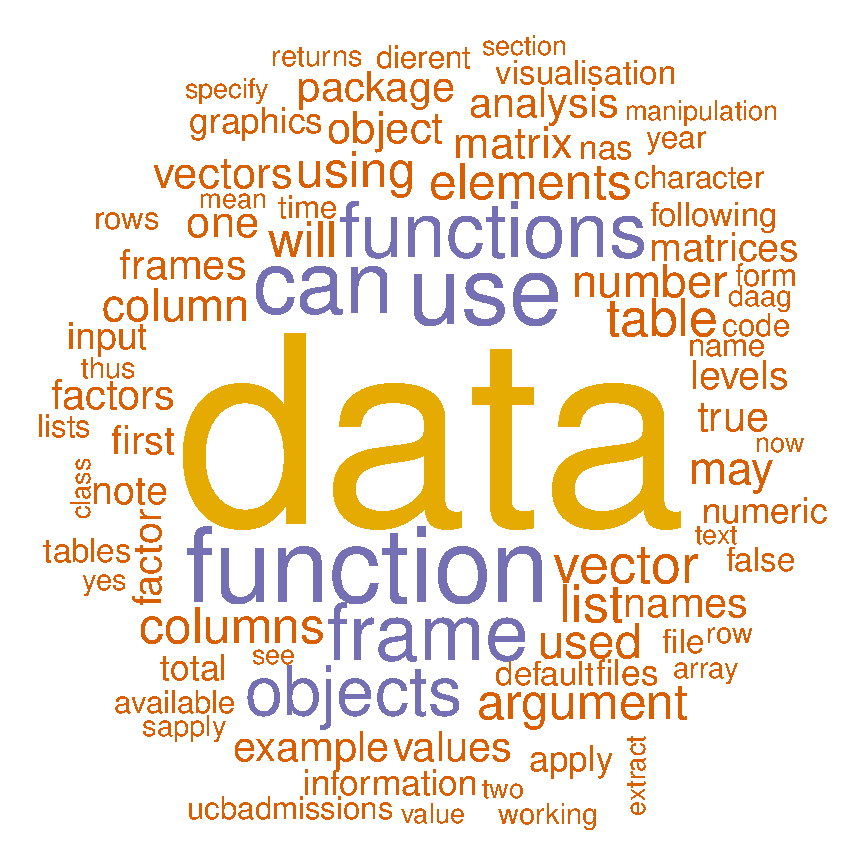
\includegraphics[width=0.32\textwidth]{figs/tm-wc-14_1x-1} 
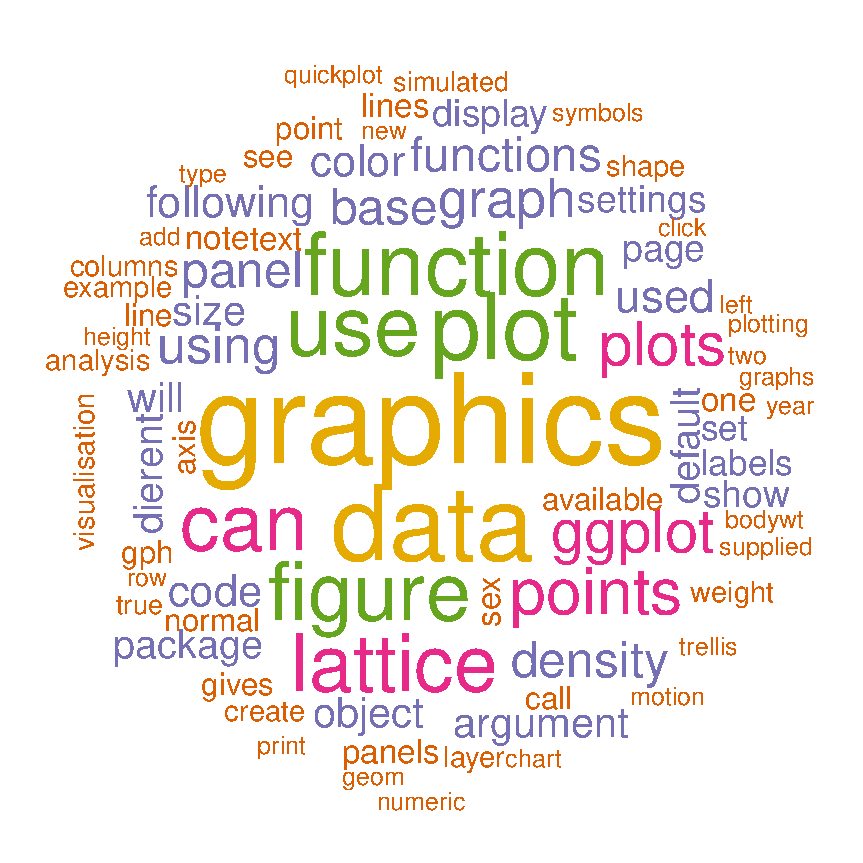
\includegraphics[width=0.32\textwidth]{figs/tm-wc-14_1x-2} 

\includegraphics[width=0.32\textwidth]{figs/tm-wc-14_1x-3} 

}



\end{knitrout}

\caption{Wordcloud plots are A: for the words in Chapters 1 - 5; B: 6 -
  7; and C: 8 - 9.\label{fig:wc}}
\end{figure}

\end{document}


